% !TEX encoding = UTF-8 Unicode
\documentclass{sig-alternate}

\usepackage{amsmath,amssymb,amsfonts,amsmath}
\usepackage{hyperref}
\usepackage{color}
\usepackage{comment}
\usepackage{mdwlist}

\includecomment{mycomment}

\hyphenation{Berle-kamp}

%%%%%%%%%%%%%%%

\newcommand{\ff}[1]{\mathbb{F}_{#1}}
\newcommand{\fq}{\ff{q}}
\newcommand{\fqn}{\ff{q^n}}

\newcommand{\dd}{d}
\newcommand{\qq}{q}
\newcommand{\QQ}{Q}
\newcommand{\nn}{n}
\newcommand{\qn}{{\qq^\nn}}
\newcommand{\extfactfdegree}{k}
\newcommand{\extfactfsize}{\qq^{\nn \cdot \extfactfdegree}}

% if we define everything in terms of base field, extension field and
% extension field used in factorization
%
\newcommand{\basef}{\ff{\qq}}
\newcommand{\extf}{\ff{\qn}}
\newcommand{\extfactf}{\ff{\extfactfsize}}

\newcommand{\AG}{\mathrm{AG}(\qq,\nn)}

\DeclareMathOperator{\Tr}{Tr}
\DeclareMathOperator{\Ker}{Ker}
\DeclareMathOperator{\Ima}{Im} 
\DeclareMathOperator{\Decomp}{Decomp} 
\DeclareMathOperator{\Var}{Var} 
\DeclareMathOperator{\Exp}{E} 
\DeclareMathOperator{\loglog}{loglog}


% to specify the number of elements of the finite fields on which the
% trace is defined
\newcommand{\tr}[2]{\Tr_{\ff{#1}:\ff{#2}}}

% to specify the number of elements of the finite fields on which the
% trace is defined: light form
\newcommand{\trl}[2]{\Tr_{#1:#2}}

% to specify the notation of the finite fields on which the trace is
% defined
\newcommand{\trabs}[2]{\Tr_{#1:#2}}
\newcommand{\trextbase}{\trabs{\extf}{\basef}}
\newcommand{\trextfactext}{\trabs{\extfactf}{\extf}}
\newcommand{\trextfactbase}{\trabs{\extfactf}{\basef}}

\newcommand{\bigO}{O}
\newcommand{\bigOt}{\tilde{O}}
\newcommand{\smallO}{o}
\newcommand{\Mul}{\mathsf{M}}

\newcommand{\Span}{\mathbf{span}}
\newcommand{\card}[1]{\# #1}
\DeclareMathOperator{\Res}{Res}

\newcommand{\cost}[1]{\color{blue}Cost:  #1\color{black}}

%%%%%%%%%%%% Algorithms

\usepackage{float,algorithm}
\usepackage[noend]{algorithmic}
\renewcommand{\algorithmicrequire}{\textbf{Input:}}
\renewcommand{\algorithmicensure}{\textbf{Output:}}

\newcounter{algo}

\newenvironment{algorithm_noendline}[4]{\begin{center}\begin{minipage}{0.48\textwidth}
      \refstepcounter{algo}
      \label{#4}
      \sf
      \rule{\textwidth}{0.2pt}\\
      \makebox[\textwidth][c]{Algorithm~\arabic{algo}:~\textbf{#1}}\\
      \rule[0.5\baselineskip]{\textwidth}{0.2pt}\\

      \vspace{-12pt}

      \parbox{\textwidth}{\textbf{Input} #2}
      \parbox{\textwidth}{\textbf{Output} #3}

\vspace{-7pt}

      \begin{enumerate*}}{\end{enumerate*}
      \vspace{-11pt}
\end{minipage}\end{center}
}

\newenvironment{algorithm_endline}[4]{\begin{center}\begin{minipage}{0.48\textwidth}
      \refstepcounter{algo}
      \label{#4}
      \sf
      \rule{\textwidth}{0.2pt}\\
      \makebox[\textwidth][c]{Algorithm~\arabic{algo}:~\textbf{#1}}\\
      \rule[0.5\baselineskip]{\textwidth}{0.2pt}\\

      \vspace{-12pt}

      \parbox{\textwidth}{\textbf{Input} #2}
      \parbox{\textwidth}{\textbf{Output} #3}

\vspace{-7pt}

      \begin{enumerate*}}{\end{enumerate*}
      \vspace{-11pt}
      \rule{\textwidth}{0.2pt}
\end{minipage}\end{center}
%\vspace{-0.5cm}
}

\floatstyle{plain}
\newfloat{algofloat}{thp}{bla}
\floatname{algofloat}{}

%%%%%%%%%%

\newcommand{\todo}[1]{\textcolor{red}{TODO: #1}}
\newcommand{\com }{\noindent \textcolor{blue}{Commentaire Micha\"el}:}
\newcommand{\comd}{\noindent \textcolor{blue}{D\'ebut Micha\"el}:}
\newcommand{\comf}{\noindent \textcolor{blue}{:Fin Micha\"el}}




\newtheorem{Def}{Definition}
\newtheorem{Theo}{Theorem}
\newtheorem{Prop}{Proposition}
\newtheorem{Lem}{Lemma}
\newtheorem{Coro}{Corollary}

\renewcommand{\paragraph}[1]{\smallskip\noindent{{\bf \rm #1.}}}

\numberofauthors{3}
\author{
  \alignauthor Luca De Feo\\
  \affaddr{Laboratoire PRiSM}\\
  \affaddr{Universit\'e de Versailles}\\
  \email{luca.de-feo@uvsq.fr}
  \alignauthor Christophe Petit\\
  \affaddr{Information Security Group}\\
  \affaddr{University College London}\\
  \email{}
  \alignauthor Micha\"el Quisquater\\
  \affaddr{Laboratoire PRiSM}\\
  \affaddr{Universit\'e de Versailles}\\
  \email{mquis@prism.uvsq.fr}
}

\title{Root-finding algorithms in small characteristic finite fields}

\begin{document}


\maketitle
\begin{abstract}
  The resolution of polynomial equations over finite fields has many
  applications, for example in cryptography or coding theory.  In this
  paper, we consider the case of polynomials over $\fqn$ where $\qq$
  is a small number.

  We revisit three algorithms to solve this problem and we describe
  their relationships in terms of the affine geometry of $\fqn$.
  Berlekamp's trace algorithm (BTA) is a classic algorithm, it
  separates the roots of $f$ based on their trace. The affine
  refinement method (ARM) separates the roots by intersecting them
  with affine subspaces. Although elegant, it is never used in
  practice since its complexity is worse than BTA. Finally, the
  successive resultant algorithm separates the roots by projecting
  them on certain other affine subspaces.

  Our contributions are four-fold. First, we provide improved variants
  of ARM and SRA, and prove that they both match the asymptotic
  complexity of BTA up to the precomputation of some finite field
  constants.  Second, we show that SRA and ARM are dual of each other
  in a precise sense.  Third, we provide several additional variants
  of our algorithms aiming at optimizing them in some special cases.
  Finally, we provide a fair experimental comparison of all
  algorithms, confirming that their complexity is equivalent in
  practice up to small constants.
\end{abstract}

\category{F.2.1}{Theory of computation}{Analysis of algorithms and problem complexity}[Computations in finite fields]
\category{G.4}{Mathematics of computing}{Mathematical software}
\terms{Algorithms,Theory}
\keywords{Finite fields, root finding, factoring.}

%%%%%%%%%%%%%%%%%%%%%%%%%%%%%%%%%%%%%%%%%%%%%%%%%%%%%%%%%%%%
%%%%%%%%%%%%%%%%%%%%%%%%%%%%%%%%%%%%%%%%%%%%%%%%%%%%%%%%%%%%
%%%%%%%%%%%%%%%%%%%%%%%%%%%%%%%%%%%%%%%%%%%%%%%%%%%%%%%%%%%%

\section{Introduction}

Let $\mathbb{F}_{\qq^\nn}$ be the finite field with $\qq^\nn$ elements, and let $f$ be a polynomial of degree $\dd$ over $\mathbb{F}_{\qq^\nn}$.
%
The \emph{root-finding problem} is the problem of computing one, several or all elements $x\in\mathbb{F}_{\qq^\nn}$ such that $f(x)=0$.
%
This problem has many applications, in particular in cryptography and in coding theory~\cite{McEliece78}. It also has a rich history, with many strategies proposed over the years. In this paper we review three related algorithms for root finding exploiting the structure of the finite affine geometry of $\extf$.



%This paper presents and compares two related algorithms for finding
%roots of polynomials with coefficients in a finite field $\extf$,
%where $\qq$ is small. The first algorithm, called the Successive
%Resultants Algorithm (SRA), was already introduced by C.~Petit
%in~\cite{cgUCL-P14}. We give here a fresh look at it and show how it
%is related to the second one. The second algorithm, called the Affine
%Refinement Method (ARM), is new, and similar in spirit to Berlekamp's
%Trace Algorithm (BTA)~\cite{berl70}.
%
%Both algorithms are deterministic. They find all the roots of a
%square-free, split polynomial of degree $\dd$ using \todo{} operations
%over $\basef$ in the worst case, and an expected \todo{} on
%average. Hence, they improve over previously known deterministic
%algorithms for root finding~\cite{Shoup91b} \todo{do they?}. For some
%parameter ranges, they also compare favorably in practice with the
%best randomized algorithms for root finding~\cite{berl70,cantor1981}.
%
%Any algorithm for root finding can be extended to an algorithm for
%factoring polynomials as mentioned in~\cite{Rabin79}. Doing so with
%our algorithms does not improve over the previous literature
%\todo{unless it does?}. However we argue in
%Section~\ref{sec:factorization} that a partial application of this
%idea yields a practical improvement to the classical Cantor-Zassenhaus
%algorithm~\cite{cantor1981}.




 

\paragraph{Previous work} %Many strategies have been proposed over the years for finding roots of polynomials defined on finite fields, and some of these methods actually solve the harder problem consisting in factoring a polynomial into its irreducible components. 
%
As mentioned by von zur Gathen~\cite{Gathen06}, the first method for finding the roots of $f \in \mathbb{F}_p[X]$, with $p$ an odd prime, is due to Legendre (1752-1833) who starts by considering the factorization of the field equation
$$X^{p}-X=X \cdot (X^{(p-1)/2}-1) \cdot (X^{(p-1)/2}+1)\,.$$
He then observes that computing the GCD of $f$ with each of the two latter factors splits the (nonzero) roots of $f$ into two sets, the squares and the non-squares. He then observes that replacing $X$ by $X+r$ for a random $r$  offers other ways of splitting the roots into two sets, which may successively be applied on the factors of $f$. This probabilistic method is the basis of many modern ones.

%In the context of coding theory, R. T. Chien~\cite{Chien64a} introduces the so-called \emph{Chien Search} in 1964. The method is essentially an exhaustive search on the roots with some optimizations for the implementation.

For a polynomial $f \in  \mathbb{F}_\qq[X]$, with $\qq$ a prime power, the factoring method of Berlekamp~\cite{berl67} is based on the so-called \emph{Petr-Berlekamp algebra} of $f$ which consists of the set of polynomials $h$ satisfying  
$$h(X)^q=h(X) \bmod{f(X)}$$
Using 
$X^{\qq}-X=\prod_{r\in \basef}(X-c)$,
Berlekamp deduces the factorization $f(X)=\prod_{r \in \mathbb{F}_{\qq}} \gcd(f(X),h(X)-r)$. The method %is deterministic and it 
requires to compute $\qq$ GCD's, hence it cannot be used for arbitrary finite fields. The root-finding method called \emph{Berlekamp Trace Algorithm} (BTA)~\cite{berl70} takes advantage of the factorization 
$$X^{\qq^n}-X=\alpha^{-1} \cdot \prod_{r \in \basef}(\tr{\qq^n}{\qq}(\alpha \cdot X)-r)\,.$$
The roots of $f$ are separated by computing GCD's with the different factors for some random $\alpha$. This method is recursive, probabilistic and may be applied to large finite fields with small characteristic. It is still one of the most efficient methods today.

Moenck~\cite{Moenck77} uses resultants to determine the $\alpha$'s and $r$'s leading to non-trivial GCD's in the above methods. He also introduces the \emph{Subgroup Refinement Algorithm} to pursue further the factorization of the field equation considered by Legendre by considering successive subgroups of $\mathbb{F}_{p}^\ast$ for some special primes $p$.
Rabin~\cite{Rabin79} proposes a method close to Legendre's. 

Cantor and Zassenhaus~\cite{cantor1981} suggests to consider random polynomials $h(X)$ instead of $X+r$ in Legendre's decomposition in order to factor a polynomial $f$ with factors of equal degree by means of GCD's. The method is probabilistic and is one the most efficient methods today.

Berlekamp~\cite{mBER84a} proposes the \emph{Least Affine Multiple method} (LAM) which consists in computing the least affine multiple of $f$, then exhaustively searching the roots of $f$ among the roots of this polynomial. 

Menezes, van Oorschot and Vanstone~\cite{MenezesOV88,OorschotV89} combines BTA with the LAM method. Moreover, they~\cite{Menvanovans92} generalize Moenck's Subgroup Refinement Algorithm~\cite{Moenck77} and 
introduce the \emph{Affine Refinement Method} (ARM) by mirroring the successive refinement of a subgroup of $\mathbb{F}_{\qq}^\ast$ in Moenck's algorithm 
by refinement of linear subspaces of $\AG$, the $\nn$-dimensional affine geometry of $\mathbb{F}_{\qq}$. %This method may be viewed as a generalization of BTA. 
As described in their papers, the ARM makes use of the LAM method.

Shoup\cite{Shoup91b} proposes a deterministic generalization of BTA for the factorization and root-finding problems. Its worst-case running time complexity is similar to the average running time of the best known probabilistic methods such as BTA and Cantor-Zassenhaus.

Niederreiter\cite{nied94} proposes an algorithm based on the resolution of differential equations over finite fields.  As mentioned by several authors~\cite{Fleis96} this algorithm is highly related Berlekamp's factoring algorithm.

%J. Bourgain  and S. Konyagin and I. Shparlinski~\cite{BKS13} propose a deterministic version of Legendre's approach for the root-finding problem of polynomials over $\mathbb{F}_p$. 

Finally, Petit\cite{cgUCL-P14} recently introduced a method called the \emph{Successive Resultants Algorithm} (SRA), that is also closely related to ARM, as we shall see.






\paragraph{Our contribution}
We review the affine refinement method (ARM), the successive resultant algorithm (SRA), Berlekamp's trace algorithm (BTA), and highlight the links between them.

The affine refinement method was designed at a time when fast arithmetic was mostly a theoretical curiosity. As pointed out in~\cite{cgUCL-P14}, the method is at best as good as BTA with fast arithmetic, and it is indeed no longer used in practice. We provide a variant of ARM that does not require the computation of the least affine multiple of $f$, and is therefore significantly more efficient. Indeed, our variant  has the same asymptotic complexity as BTA, up to constant factors and some precomputation (which is also present in the original algorithm); whereas the original method is only interesting for very small degree polynomials. It also has the same complexity as SRA.

With respect to the original paper~\cite{cgUCL-P14}, our variant of the successive resultant algorithm adds a squarefree reduction step in the last loops of the first phase to reduce the degrees of the polynomials involved. This enables early termination of the algorithm, which is especially effective on large degree polynomials. We also introduce an ad hoc algorithm to perform the special resultant computations required by SRA, and we compute the roots in the second step with multi-evaluation rather than by solving small degree equations. Put together, our modifications improve slightly the asymptotic complexity, and give an algorithm efficient and easier to implement.

We also provide methods to decrease the precomputation costs of both methods significantly when the field extension degree is composite, and a method to reduce it down to the cost of the other steps in the case of ARM.

Finally, we show that SRA and ARM are in a sense dual of each other, and that our precomputation-free variant of ARM is in fact a generalized version of BTA.

\paragraph{Outline}
The paper is organized as follows. In Sec 2 we review basic facts
about the finite affine geometry $\AG$. In Sec 3 we present the three
root finding algorithms based on the structure of $\AG$: ARM, SRA and
BTA. In Sec 4 we present some refinements of those algorithms, that
apply in special cases. In Sec 5 we present experimental
results.


\section{The affine geometry AG(\qq,\nn)}
\label{sec:nsd}

% $\AG$

The main ingredient of the algorithms we present is the \emph{finite
  affine geometry} $\AG$, i.e., the set of all vector subspaces of
$\basef^\nn$ and their translates. Fixing a basis
of $\extf$ over $\basef$, we can
identify the elements of $\extf$ with the points of $\AG$. The
relationship between $\AG$ and the problem of root finding was
originally highlighted in~\cite{OorschotV90}.

\paragraph{Approximating $\extf$ by a flag} Let
$\{\upsilon_1,\ldots,\upsilon_\nn\}$ be any basis of
$\extf/\basef$. To this basis, we associate the flag of linear
subspaces $V_0\subset V_1\subset \cdots \subset V_\nn$ defined by
\begin{equation}
  V_i = \Span(\upsilon_1,\dots,\upsilon_i),
\end{equation}
so that $\dim V_i = i$ and $\card V_i = \qq^i$. To each of the
subspaces we associate its minimal polynomial, that we denote by
$L_i$. Then we have the well know relation (see~\cite[Ch. 11]{mBER84a})
\begin{equation}
\label{Li_generation}
  L_0(X) = X, \; \;  L_i(X) = (X^\qq - L_{i-1}(\upsilon_i)^{\qq-1}X)\circ L_{i-1}(X),
\end{equation}
and in particular $L_\nn=X^\qn-X$.

Notice that, by definition, each $L_i$ defines a linear map
$\extf\to\extf$, with kernel $V_i$. It will be convenient to encode
this information in an $\nn\times\nn$ matrix, thus we define
$\gamma_{i,j}=L_i(\upsilon_j)$, and
\begin{equation}
  \label{eq:Gamma}
  \Gamma =
  \begin{pmatrix}
    \gamma_{0,1} & \cdots & \gamma_{0,\nn}\\
    \vdots & & \vdots\\
    \gamma_{\nn-1,1} & \cdots & \gamma_{\nn-1,\nn}
  \end{pmatrix}.
\end{equation}
Observe that by definition $\gamma_{i,j}=0$ whenever $j\le i$, hence
$\Gamma$ is an upper triangular matrix, associated to a linear map
$\extf\to\extf^\nn$ sending any $\delta\in\extf$ to the vector
$\bigl(L_0(\delta),\dots,\allowbreak L_{n-1}(\delta)\bigr)$.  

Now define $V_i^\ast$ as the image space of $L_i$, i.e., the subspace
generated by the elements of the $i$-th row of $\Gamma$.  It is easily verified that
$\dim V_i^\ast=n-i$ and that $\{\gamma_{i,i+1},\dots,\gamma_{i,\nn}\}$
is a basis. Then define $L_i^\ast$ as the minimal polynomial of
$V_i^\ast$. It is shown in~\cite[Ch. 11]{mBER84a} that
$L_i^\ast$ is the unique linearized polynomial such that
\begin{equation}
\label{dual_polynomial}
(L_i^\ast \circ L_i)(X)=(L_i \circ L_i^\ast)(X)=X^\qn-X\,,
\end{equation}
where $L_i^\ast$ is called the \emph{dual} of $L_i$.

\begin{Lem}
  \label{lem:gamma}
  The coefficients of the matrix $\Gamma$ can be computed using
  $O(\nn^2\log\qq)$ operations over $\extf$.
\end{Lem}
\begin{proof}
  By the recursive definition of $L_i$, it is clear that
  \begin{equation}
    \gamma_{i,j} =
    \begin{cases}
      \upsilon_j &\text{for $i=0$},\\
      \gamma_{i-1,j}^\qq - \gamma_{i-1,i}^{\qq-1}\gamma_{i-1,j} &\text{for $i>0$}.
    \end{cases}
  \end{equation}
  Thus, each $\gamma_{i,j}$ can be computed from the previous ones
  using $O(\log\qq)$ operations, and there is a total $O(\nn^2)$ of
  them to compute.
\end{proof}

The eigenvalues of $\Gamma$ play a special role in our algorithms,
thus we define $\beta_i=\gamma_{i-1,i}$ and $\alpha_i=\beta_i^{\qq-1}$
for any $1\le i \le \nn$. We deduce a decomposition
\begin{equation}
\label{decomposition_field_eq_gen}
  X^\qn - X = (X^\qq - \alpha_\nn X) \circ \cdots \circ (X^\qq - \alpha_1 X).
\end{equation}

\paragraph{The affine geometry of $\extf$} 
Let now $\rho\in\extf$, such that $\rho=\sum_jr_j\upsilon_j$.  For any
$V_i$ we define the affine space (also called an $i$-flat)
\begin{equation}
  V_{i,\rho} = V_i + \rho.
\end{equation}
By construction, the reunion of all $i$-flats for any $i$ is
isomorphic to $\AG$, and we call it the \emph{affine geometry of
  $\extf$}. We also define the polynomial $M_{i,\rho}$ as the minimal
polynomial of $V_{i,\rho}$, hence
\begin{equation}
  M_{i,\rho}(X) = L_i(X - \rho) = L_i(X) - \sum_{j>i}r_j\gamma_{i,j}.
\end{equation}
Observe that $M_{i,\rho}=M_{i,\rho'}$, and thus
$V_{i,\rho}=V_{i,\rho'}$, if and only if $\rho-\rho'\in V_i$. Hence
any $V_{i,\rho}$ can be represented canonically by taking $\rho$ of
the form $\rho=\sum_{j>i}r_j\upsilon_j$. Hence there are exactly
$\qq^{n-i}$ distinct $i$-flats, each of size $\qq^i$.

By definition we have
\begin{equation}
  V_{i,\rho} = \bigcup_{c\in\basef} V_{i-1,\rho + c\upsilon_i},
\end{equation}
hence
\begin{equation}
\label{node_product}
  M_{i,\rho}(X) = \prod_{c\in\basef} M_{i-1,\rho+c\upsilon_i}(X).
\end{equation}
This defines a decomposition of $X^{\qn}-X$ into a product tree, where
each node at level $i$ is a $M_{i,\rho}$, defined by a
$\rho=\sum_{j>n-i}r_j\upsilon_j$, and has $\qq$ children, defined by
the elements $c\upsilon_{n-i}+\rho$ for $c\in\basef$. In particular,
the leaves are the linear polynomials $X-\rho$ for all points
$\rho\in\extf$.



\section{Root finding using  AG(\qq,\nn)}
\label{sec:arm-sra}

%$\AG$

We are interested in algorithms for the following problem: given a
degree $\dd$ polynomial $f(X)$ with coefficients in a finite field
$\extf$, find all the roots $\rho\in\extf$ such that $f(\rho)=0$.  In
this section, we present algorithms based on the structure of the
affine geometry described previously.

\subsection{Preliminaries}

\paragraph{Complexity notations} In this paper, we use an
\emph{algebraic complexity model}, where the running time of an
algorithm is measured in terms of the number of operations ($+$,
$\times$, $\div$) in $\extf$, and its space requirements in terms of
number of elements of $\extf$ stored. As customary, we use the
$\bigO$-notation to neglect constant factors. All asymptotic
complexities will be expressed in terms of the parameters $\qq$, $\nn$
and $\dd$.

We denote by $\Mul : \mathbb{N} \to \mathbb{N}$ a function such that
polynomials in $\extf[X]$ of degree at most $m$ can be multiplied in
$\Mul(m)$ operations ($+$, $\times$) in $\extf$, and we make the
usual super-linearity assumptions on
$\Mul$~\cite[Chapter~8]{Gathen2003}.  Using FFT multiplication, we can
take $\Mul(m)\in\bigO(m \log m \loglog m)$.

\paragraph{Fundamental algorithms}
%
%\todo{I (CP) would move this section as subsection 2.1. The current subsection 2.1 will then become section 2.2, or maybe section 3.}
%
We recall now the complexities of the basic subroutines we shall need next.
%
The greatest common divisor of two polynomials of degree $\dd$ can be computed in $\bigO(\Mul(\dd)\log \dd)$ operations in $\extf$ using a Sch\"on\-hage-type algorithm~\cite{Schoenhage1971,Thull1990}.
%
Interpolating a polynomial of degree $\dd$ from $\dd+1$ points can be done in $O(\Mul(\dd)\log\dd)$ operations using the algorithm described in~\cite[Ch. 10]{Gathen2003}. Similarly, evaluating a polynomial of degree $\dd$ at $\dd+1$ points can also be done in $\bigO(\Mul(\dd)\log \dd)$ operations using the multi-point evaluation algorithm of~\cite[Ch. 10]{Gathen2003}.

In root-finding literature, it is common to assume that all the irreducible factors of the polynomial are linear and distinct. This can be enforced by replacing $f(X)$ with $\gcd(X^\qn-X,f(X))$. The main cost of this GCD is the computation of $X^\qn\bmod f(X)$. This can be achieved with a standard square-and-multiply algorithm in $O(\nn\Mul(\dd)\log q)$, or (when $\nn$ is large) via modular composition (see~\cite{GathenS92,Kedlaya11}). 


%In the last case, the best algorithm asymptotically is due to Kedlaya and Umans~\cite{Kedlaya2011} and requires $\bigO(\dd^{1.5+o(1)}\log^{1+o(1)}\qq^\nn+\dd^{1+o(1)}\log^{2+o(1)}\log \qq^\nn)$ bit operations.

%, or with a more involved iterated Frobenius algorithm~\cite{Gathen1992}.

Recall that, given polynomials $f$ and $g$, the resultant
$$\Res_X(g(X)-Y,f(X))$$
has the same degree as $f$, and its roots are the elements $g(\rho)$
for each root $\rho$ of $f$, taken with multiplicity. We shall need an
algorithm to compute a special resultant of this kind:
$$\Res_X(X^\qq-\beta^{\qq-1}X-Y,f(X))$$
for some $\beta\in\extf$. This is described in
Algorithm~\ref{alg:resultant}, and relies upon the variant of
multi-point evaluation described in Algorithm~\ref{alg:multi-ev}.



\begin{algorithm}
  \caption{Polynomial evaluation at special points}
  \label{alg:multi-ev}
  \begin{algorithmic}[1]
    \REQUIRE A polynomial $f\in\extf[X]$ of degree $\dd$,\\
    $\delta_0,\dots,\delta_\dd\in\extf$ and $\beta\in\extf$.
    \ENSURE $f(\delta_i+c\beta)$ for all $0\le i \le \dd$ and $c\in\basef$.
    \STATE Let $\alpha = \beta^{\qq-1}$;
    \STATE\label{alg:multi-ev:mod} Compute $\bar{f}(X,Y) = f \mod X^\qq-\alpha X-Y$;
    \STATE Let $\bar{f}(X,Y) = \sum_j \bar{f}_j(Y)X^j$;
    \STATE\label{alg:multi-ev:Delta} Compute $\Delta_i=\delta_i^\qq-\alpha\delta_i$ for $0\le i\le\dd$;
    \FOR {$0\le j<\qq$}
    \STATE\label{alg:multi-ev:multi-ev} Compute $\eta_{i,j}=\bar{f}_j(\Delta_i)$ for $0\le i\le\dd$;
    \ENDFOR
    \STATE Let $f_i(X) = \sum_j \eta_{i,j}X^j=\bar{f}(X,\Delta_i)$;
    \FOR {$0\le i \le\dd$}
    \STATE\label{alg:multi-ev:final-ev} Compute $\varepsilon_{i,c}=f_i(\delta_i+c\beta)$ for all $c\in\basef$;
    \ENDFOR
    \RETURN $\varepsilon_{i,c}$ for $0\le i\le\dd$ and $c\in\basef$.
  \end{algorithmic}
\end{algorithm}

\begin{Lem}
  \label{lem:multi-ev}
  Algorithm \ref{alg:multi-ev} is correct. On input a polynomial of
  degree $\dd\gg\qq$ and $O(\dd)$ evaluation points, it computes its
  output using $O(\Mul(\dd) \log\dd + \qq^2\Mul(\dd/\qq)\log\dd +
  \qq^2\dd)$ operations over $\extf$.
\end{Lem}
\begin{proof}
  Observe that
  $\prod_{c\in\basef}(X-\delta_i-c\beta)=X^\qq-\alpha X-\Delta_i$, with
  $\Delta_i$ defined as in step~\ref{alg:multi-ev:Delta}. Hence
  \begin{equation*}
    f_i(X)=f(X)\mod \prod_{c\in\basef}(X-\delta_i-c\beta)
  \end{equation*}
  Correctness follows immediately.

  We now analyze the complexity. In step~\ref{alg:multi-ev:mod}, we
  reduce $f$ so that $\bar{f}$ has degree $<\qq$ in $X$. This
  reduction can be computed in $O(\Mul(d)\log d)$ using a
  divide-and-conquer approach.

  By construction, the polynomials $\bar{f}_j(Y)$ have degree
  $O(\dd/\qq)$, hence step~\ref{alg:multi-ev:multi-ev} can be computed
  in $O(\qq\Mul(\dd/\qq)\log\dd)$ splitting the points $\Delta_i$ in
  $q$ batches, and using $\qq$ classical multi-point
  evaluations. Hence, the overall cost of the for loop is
  $O(\qq^2\Mul(\dd/\qq)\log\dd)$.

  Finally, step~\ref{alg:multi-ev:final-ev} can be computed again by
  multipoint evaluation in degree $O(\qq)$. However, we assume that
  $\qq$ is too small, to apply an asymptotically fast algorithm, thus
  we account $O(\qq^2)$ operations for this step, giving $O(\qq^2\dd)$
  operations for the whole loop. All other steps have negligible cost.
\end{proof}

\begin{algorithm}
  \caption{Resultant with a special polynomial}
  \label{alg:resultant}
  \begin{algorithmic}[1]
    \REQUIRE A polynomial $f\in\extf[X]$ of degree $\dd<\qq^{n-1}$,\\
    an element $\beta\in\extf$.
    \ENSURE The resultant $\Res_X\bigl(X^\qq-\beta^{\qq-1}X-Y,f(X)).$
    \STATE Let $\alpha=\beta^{\qq-1}$,
    \STATE\label{alg:resultant:select} Select points $\delta_0,\dots,\delta_d$ s.t. all $\delta_i^\qq-\alpha\delta_i$ are distinct;
    \STATE\label{alg:resultant:multi-ev} Compute $\varepsilon_{i,c}=f(\delta_i+c\beta)$ for $0\le i\le\dd$ and $c\in\basef$;
    \RETURN\label{alg:resultant:interp} $g$ such that $g\left(\prod_c\delta_i+c\beta\right) = (-1)^{\qq\dd}  \prod_c\varepsilon_{i,c}$.
  \end{algorithmic}
\end{algorithm}


\begin{Lem}
  \label{lem:alg-resultant}
  Algorithm~\ref{alg:resultant} is correct. On input a polynomial of
  degree $d\ll\qq^{\nn-1}$, it computes its output using $O(\Mul(\dd)
  \log\dd + \qq^2\Mul(\dd/\qq)\log\dd + \qq^2\dd)$ operations over
  $\extf$.
\end{Lem}
\begin{proof}
  It is well known that the resultant commutes with evaluation, i.e., if
  \begin{equation}
    g(Y) = \Res_X\bigl(X^\qq-\beta^{\qq-1}X-Y,f(X)\bigr),
  \end{equation}
  then
  \begin{equation}
    g(\Delta) = \Res_X\bigl(X^\qq - \beta^{\qq-1}X -\Delta , f(X)\bigr)
  \end{equation}
  for any $\Delta\in\extf$. Our algorithm is just a specialization of
  the classical evaluation-interpolation approach to compute bivariate
  resultants. We know that the polynomial $g$ has degree $\dd$, thus
  we only need to evaluate at $d+1$ points.

 % To make things simpler, we start by changing the sign of the right
  %operand, setting
  %\begin{equation}
  %  h(Y) = \Res_X\bigl(X^\qq-\beta^{\qq-1}X-Y, f(X)\bigr) = (-1)^\dd g(Y).
  %\end{equation}
  Let now $\delta\in\extf$ be such that
  $\Delta=\delta^\qq-\beta^{\qq-1}\delta$. By linearity we have
  \begin{multline}
    \label{eq:lin-resultant}
    \Res_X\bigl(X^\qq-\beta^{\qq-1}X-\Delta,f(X)\bigr) =\\
    \Res_X\Bigl(  \prod_{c\in\extf}(X-\delta - c\beta),f(X) \Bigr) =\\
    \prod_{c\in\extf} \Res_X\bigl(X-\delta - c\beta, f(X)\bigr) =\\
    (-1)^{\qq\dd} \prod_{c\in\extf} f(\delta+c\beta),
  \end{multline}
  where the second and third equalities come from the
  multiplicativity of the resultant. The correctness of the algorithm
  now follows immediately.

  We now go to the complexity. The interpolation points at
  step~\ref{alg:resultant:select} can be selected at random, keeping
  track of the values $\Delta_i=\delta_i^\qq-\beta^{\qq-1}\delta_i$,
  and discarding duplicates. If $\dd\ll\qq^{n+1}$, we are likely to
  find enough points in $O(d)$
  tries. Step~\ref{alg:resultant:multi-ev} is computed using
  Algorithm~\ref{alg:multi-ev}, at the cost given in
  Lemma~\ref{lem:multi-ev}. Finally, step~\ref{alg:resultant:interp}
  is computed using a classical fast interpolation algorithm, at a
  cost $O(\Mul(d)\log d)$.
\end{proof}

Observe that the condition in Algorithm~\ref{alg:resultant} of having
$\dd+1$ points $\delta_i$ such that
$\Delta_i=\delta_i^\qq-\beta^{\qq-1}\delta_i$ are all distinct can
only be verified if $\dd+1\le\qq^{\nn-1}$. If more interpolation
points are needed, Eq.~\eqref{eq:lin-resultant} cannot be applied
anymore, but the evaluation-interpolation approach is still possible
at a slightly worse cost. However, this is not a major concern for the
algorithms we present next.



\subsection{Two variants of ARM and SRA}

We now present our variants of two root finding algorithms based on
the structure of $\AG$. We start with the Affine
Refinement Method (ARM) of Menezes, van Oorschot and
Vanstone~\cite{Menvanovans92}, then go to the Successive Resultants
Algorithm (SRA) of Petit~\cite{cgUCL-P14}. For both, we present
variants which are more efficient than the original ones. Our
presentation highlights a link between the two algorithms that had
previously gone unnoticed: in both an abstract and a computational
sense, ARM and SRA can be seen as \emph{dual} to each other.

ARM works by \emph{intersecting} the roots of the input polynomial
with the subspaces $V_{i,\rho}$. The successive intersections are
computed by means of GCDs.  SRA works by \emph{projecting} the roots
onto the spaces $V_i^\ast$.  The successive projections are computed
by means of resultants.

At an algorithmic level, the duality is embodied in the well known
property
\begin{equation}
  \gcd\bigl(f(X),g(X)\bigr) \ne 1 \;\Leftrightarrow\; \Res_X\bigl(f(X),g(X)\bigr)=0\,,
\end{equation}
which implies that ARM isolates a root of $f$ whenever SRA does.

\paragraph{Pre-computation} Both methods take as input a basis
$\upsilon_1\dots,\upsilon_\nn$, and use it to define the affine space
$\AG$ as in Section~\ref{sec:nsd}. To this end, they compute the
matrix $\Gamma$ of Eq.~\eqref{eq:Gamma} at a cost of $O(n^2\log q)$
operations. Note that this phase depends only on the field and may be
re-used for the root-finding of several polynomials defined on the
same field.

\paragraph{ARM} The method consists in \emph{intersecting} the roots of $f$ with the $i$-flats  $V_{i,\rho}$, i.e, with the fibers by $L_i$ of each element $\ell_{i,\rho} \in V_i^\ast$.
%The method consists in \emph{projecting} the roots of $f$ onto the spaces $V_i^\ast$ while simultaneously \emph{intersecting} those with the corresponding fibers of $L_i$ identified by $\ell_i$.
 This is achieved by computing the non-constant GCDs among the set
% the computation of the minimal polynomial of those intersections by means of gcd's, i.e. 
 \begin{equation}
 \label{base_ARM}
\gcd(L_i(X)-\ell_{i,\rho},f(X))     \mbox{ for any }  \ell_{i,\rho}  \in V_i^\ast\,,
\end{equation}
for $i$ starting from $n$ and going down to 0.
It ultimately leads to the roots of $f$ because the GCD's satisfying
$$\gcd(L_0(X)-\ell_{0,\rho},f(X))=\gcd(X-\ell_{0,\rho},f(X)) \ne 1$$ 
yield the linear factors of $f$. 
Note that 
\begin{equation}
  \label{eq:duality-gcd}
  \gcd(L_i(X)-\ell_{i,\rho},f(X)) \ne 1
\end{equation}
implies that there is a root of $f$ in $V_{i,\rho}$.
In practice, these GCDs are computed in a recursive way. Let us first define
 $$f_{i,\rho}(X)=\gcd(L_i(X)-L_i(\rho),f(X))\,$$
where $\rho \in \extf$. Hence $f_{i,\rho}(X)=f_{i,\rho'}(X)$ if and only if $\rho-\rho' \in V_i$.
Using Eq.~\eqref{base_ARM} and the fact that $V_n^\ast=\{0\}$, $f_{n,0}(X)$ is first computed, i.e.,
 $$f_{n,0}(X)=\gcd(L_n(X),f(X))=\gcd(X^{q^\nn}-X,f(X))\,.$$
The recursive step is based on Eq.~\eqref{node_product} and works as follows: for any $L_i(\rho) \in V_i^\ast$ such that $f_{i,\rho}(X)$ is neither a constant polynomial nor a linear factor,
  $$
  \begin{array}{lll}
  f_{i,\rho}(X)&=&\prod_{c \in \basef} \gcd(M_{i-1,\rho+c \cdot \upsilon_i}(X),f_{i,\rho}(X)) \\
               &=&\prod_{c \in \basef} \gcd(L_{i-1}(X)-L_{i-1}(\rho+c \cdot \upsilon_i),f_{i,\rho}(X)) \\
               &=&\prod_{c \in \basef} f_{i-1,\rho+c \cdot  \upsilon_i}(X)\\
  \end{array}              
  $$ 
 
 This procedure builds a tree where at each level only the nodes containing a polynomial of degree strictly greater than 1 have children. Said otherwise, the leafs of the tree are either constant polynomials or the distinct linear factors of $f$ (without their algebraic multiplicity). ARM is summarized in Algorithm~\ref{alg:arm}.

%Note that the $l_i$ for which $\gcd(f(X),L_i(X)-l_i) \ne 1$ correspond to the $L_i$-projections onto $V_i^\ast$ of the roots of $f$.
  
 \begin{algorithm}
   \caption{Affine Refinement Method}
   \label{alg:arm}
   \begin{algorithmic}[1]
   \REQUIRE {A polynomial $f\in\extf[X]$ of degree $\dd$,\\
     A basis $\upsilon_1,\dots,\upsilon_\nn$ of $\extf$,\\
     The matrix $\Gamma=(\gamma_{i,j})$ defined in~\eqref{eq:Gamma}.}
   \ENSURE {The roots of $f$ in $\extf$.}
   \STATE Set $L_0 = X$;
   \FOR {$1 \le i \le \nn$}
   \STATE\label{alg:arm:Li} Compute $L_i = L_{i-1}^\qq - \gamma_{i-1,i}^{\qq-1} L_{i-1} \mod f$;
   \ENDFOR
   \STATE Initialize tree with root $f_{\nn,0} = f \mod L_\nn$;
   \FOR {$\nn \ge i \ge 1$}\label{alg:arm:for}
   \FOR {any node $f_{k,\rho}$ of degree $>1$ in the tree}
   \STATE\label{alg:arm:combili} Compute $\ell_{i-1,\rho} = L_{i-1}(\rho) = \sum_j r_j\gamma_{i-1,j}$;
   \ENDFOR
   \FOR {any leaf in the tree $f_{i,\rho}$ of degree $>1$}
   \STATE\label{alg:arm:mod} Compute $\bar{L}_\rho = L_{i-1}\mod f_{i,\rho}$;
   \FOR {any $c\in\basef$}
   \STATE\label{alg:arm:gcd} $f_{i-1,\rho+c\cdot \upsilon_i} = \gcd(\bar{L}_\rho - \ell_{i-1,\rho} - c\gamma_{i-1,i}, f_{i,\rho})$;
   \ENDFOR
   \ENDFOR
   \IF {all leaves have degree $\le 1$}
   \RETURN The root of each leaf of degree $1$.
   \ENDIF
   \ENDFOR
   \end{algorithmic}
 \end{algorithm}

 \begin{Lem}
 \label{complexity_arm}
   Algorithm~\ref{alg:arm} (ARM) is correct. If the root tree for the
   input $f$ and $\upsilon_1,\dots,\upsilon_\nn$ has height $h$, it
   computes its output using $O(\nn\Mul(\dd)\log\qq + h^2\dd +
   h\qq\Mul(\dd)\log\dd)$ operations over $\extf$.
 \end{Lem}
 \begin{proof}
   Correctness has been discussed above. Concerning complexity, the
   computation of the polynomials $L_i$ in step~\ref{alg:arm:Li} is
   done in $O(\Mul(\dd)\log\qq)$ for each polynomial, contributing
   $O(\nn\Mul(\dd)\log\qq)$ to the total.

   Now we treat the steps inside loop~\ref{alg:arm:for}.  Each of the
   complexities below is multiplied by $h$ in the total count.

   In step~\ref{alg:arm:combili}, we need to compute $L_{i-1}(\rho)$
   for each root approximation $\rho$ in the tree. If $\rho$ is the
   approximation associated to a node, and $\rho'$ is the
   approximation associated to its parent, then
   $\rho-\rho'=c\upsilon_j$ for some $c\in\basef$ and some basis
   vector $\upsilon_j$. Hence, knowing the elements $\gamma_{i-1,j}$,
   the value $L_{i-1}(\rho)$ can be computed from $L_{i-1}(\rho')$
   using only one field operation. At any iteration, there are at most
   $hd$ nodes in the tree, hence a cost of $O(hd)$.

   Step~\ref{alg:arm:mod} can be computed putting all $f_{i,\rho}$
   together in a subproduct tree, as in the classical multi-point
   evaluation algorithm. Reducing modulo the subproduct tree costs
   then $O(\Mul(\dd)\log\dd)$.

   Finally, in step~\ref{alg:arm:gcd} the degrees of the polynomials
   $f_{i,\rho}$ sum up to $\dd$. For each of these, we compute $\qq$
   GCDs with polynomials of similar degree. Each of these polynomials
   can be computed in $O(\Mul(\dd_\rho)\log\dd_\rho)$, where
   $\dd_\rho$ is the degree of $f_{i,\rho}$. Summing over all
   polynomials, and using the super-linearity of the function $\Mul$,
   we bound this by $O(\qq\Mul(d)\log d)$.
 \end{proof}

\paragraph{SRA} The method consists in \emph{projecting} the roots of $f$ onto the spaces $V_i^\ast$ for $i$ starting from $n$ and going down to 0.
It is achieved by the computation of the values $\ell_{i,\rho} \in V_i^\ast$ annihilating
 \begin{equation}
 \label{base_SRA}
\Res_X(L_i(X)-\ell_{i,\rho},f(X)) \,.
\end{equation}
It ultimately leads to the roots of $f$ because
$$\Res_X(L_0(X)-\ell_{0,\rho},f(X))=\Res_X(X-\ell_{0,\rho},f(X))=0\,$$
means that $\ell_{0,\rho}$ is a root of $f$. Note that 
\begin{equation}
  \label{eq:duality-res}
  \Res_X(L_i(X)-\ell_{i,\rho},f(X)) =0
\end{equation}
means that there is a root of $f$ in $V_{i,\rho}$.  Comparing this
with Eq.~(\ref{eq:duality-gcd}), the duality between ARM and SRA
becomes apparent. Indeed, $\gcd(L_i(X)-\ell_{i,\rho},f(X)) \ne 1$ if
and only if $\Res_X(L_i(X)-\ell_{i,\rho},f(X)) =0$.

Like ARM, SRA is a two-swipes algorithm.  We first compute the
polynomials $f^{(i)}$ having as roots the projections onto $V_i^\ast$
of the roots of $f$, i.e.,
\begin{equation}
\label{original_resultant}
f^{(i)}(Y_i)=\Res_{X}(L_i(X)-Y_i,f(X))  \mbox{ for } 0\le i\le n \,.
\end{equation}
The polynomial $f^{(i)}$ is computed from $f^{(i-1)}$ by projecting
its roots onto $V_i^\ast$. By the definition of $L_i$, we have  $f ^{(0)}=f$ and
$$f^{(i)}(Y_i)=\Res_{X_{i-1}}(X^q_{i-1} - \alpha_i X_{i-1} -Y_i,f^{(i-1)}(X_{i-1})) \,.$$

At each iteration, some roots of $f^{(i-1)}$ may be projected to the
same root of $f^{(i)}$. We apply a square-free factorization algorithm
to only keep one representative of those roots. Doing this allows us
to stop the descent before $f^{(n)}$ is computed. Indeed, we can
verify that $f^{(i)}=L_i^\ast$ simply by checking the degree of
$f^{(i)}$, then we know that the roots of $f^{(i)}$ are all the
elements of $V_i^\ast$. In the worst case, this will happen at the
last step, when $f^{(n)}(X)=X=L_n^\ast(X)$, and the only root is $0$.
In practice, the square-free factorization is unlikely to
significantly reduce the degree of $f$ before the last $\log\dd$
iterations, it is thus advisable to skip it in the first ones.

After the $f^{(i)}$'s are computed, SRA iteratively computes their
roots starting from the last. The roots of $f^{(i-1)}$ are deduced
from those of $f^{(i)}$ using Eq.~\eqref{Li_generation}. For any root
$\ell_i$ of $g^{(i)}$ belonging to $V_i^\ast$, we check whether
$g^{(i-1)}(\ell_{i-1})=0$ for any $\ell_{i-1} \in V_{i-1}^\ast$ such that
$\ell_{i-1}^\qq-\alpha_i \cdot \ell_{i-1}=\ell_i$. This procedure builds
a tree where at level $i$ the nodes are the roots of $g^{(i)}$.  The
leafs of the tree at level $0$ are the roots of $f$.

  
 \begin{algorithm}
   \caption{Successive Resultant Algorithm}
   \label{alg:sra}
   \begin{algorithmic}[1]
   \REQUIRE {A polynomial $f\in\extf[X]$ of degree $d$,\\
     A basis $\upsilon_1,\dots,\upsilon_\nn$ of $\extf$,\\
     The matrix $\Gamma=(\gamma_{i,j})$ defined in~\eqref{eq:Gamma}.}
   \ENSURE {The roots of $f$ in $\extf$.}
   \STATE Let $f^{(0)}=f$;
   \FOR {$1\le i \le \nn$}\label{alg:sra:for1}
   \STATE\label{alg:sra:resultant} $\hat{f}^{(i)}(Y) = \Res_X(X^\qq - \gamma_{i-1,i}^{\qq-1}X-Y,f^{(i-1)}(X))$;
   \STATE\label{alg:sra:sqfree} Compute $f^{(i)}$, the square-free part of $\hat{f}^{(i)}$;
   \IF{$\deg f^{(i)} = \qq^{\nn-i}$}
   \STATE  \label{alg:sra:condition:res}  Set $h=i$;
   \STATE {\bf break} out of the {\bf for} loop;
   \ENDIF
   \ENDFOR
   \STATE Let $A_h = (\rho_0,\dots,\rho_{\qq^{\nn-h}})$ such that $V^\ast_h=\bigl(L_h(\rho_j)\bigr)_j$;
   \FOR {$h> i\ge 0$}\label{alg:sra:for2}
   \FOR {any $\rho\in A_i$}
   \STATE\label{alg:sra:combili} Compute $\ell_{i,\rho}=L_i(\rho)=\sum_jr_j\gamma_{i,j}$;
   \ENDFOR
   \STATE\label{alg:sra:eval} $E_i = \left(f^{(i)}(\ell_{i,\rho} + c\gamma_{i,i+1}) \text{ for any $\rho\in A_{i+1}$ and $c\in\basef$}\right)$;
   \FOR {any $\rho\in A_i$}
   \STATE Add $\rho+c\upsilon_{i+1}$ to $A_i$ only if $f^{(i)}(\rho+c\gamma_{i,i+1})=0$.
   \ENDFOR
   \ENDFOR
   \RETURN $A_0$.
   \end{algorithmic}
 \end{algorithm}

 \begin{Lem}
 \label{complexity_sra}
   Algorithm~\ref{alg:sra} (SRA) is correct. If the root tree for the
   input $f$ and $\upsilon_1,\dots,\upsilon_\nn$ has height $h$, it computes its
   output using $O\left(h(\Mul(\dd)\log \dd +
     \qq^2\Mul(\dd/\qq)\log\dd + \qq^2\dd + h\dd)\right)$ operations
   over $\extf$, or more compactly $O(h\qq\Mul(\dd)\log\dd + h^2\dd)$.
 \end{Lem}
 \begin{proof}
   Correctness has been discussed above. Concerning complexity, we
   remark that any step in loop~\ref{alg:sra:for1} and
   loop~\ref{alg:sra:for2} is repeated exactly $h$ times, thus the
   overall complexity is multiplied by $h$.

   Step~\ref{alg:sra:resultant} can be computed using
   Algorithm~\ref{alg:resultant}. According to
   Lemma~\ref{lem:alg-resultant}, this costs $O(\Mul(\dd) \log\dd +
   \qq^2\Mul(\dd/\qq)\log\dd + \qq^2\dd)$.

   Step~\ref{alg:sra:sqfree} is computed in $O(\Mul(\dd)\log\dd)$ using
   a classical algorithm.

   The elements $L_i(\rho)$ in step~\ref{alg:sra:combili} are computed
   using the tree structure of the roots, like in ARM, thus requiring
   only one field operation per value. There are at most $hd$
   approximations at each iteration, thus this step contributes
   $O(hd)$ operations.
   
   Finally, step~\ref{alg:sra:eval} can be computed using the
   multi-point evaluation algorithm~\ref{alg:multi-ev}, at the same
   cost of step~\ref{alg:sra:resultant}.
 \end{proof}
   
  
%  \underset{n \to +\infty}{\overset{w^*}{\longrightarrow}}0
 Using the two previous lemmas, we can now easily state the worst case
 complexity of both ARM and SRA, indeed for both algorithms the height
 $h$ equals $\nn$ in this case. Unsurprisingly, the two algorithms
 have very similar complexities.

 \begin{Theo}
   In the worst case, both ARM and SRA compute their output using
   $O(nq\Mul(d)\log d + n^2d)$.
 \end{Theo}
 
 
 
 
 \subsection{BTA}
\label{sec:bta}

For completeness, we review here Berlekamp's trace algorithm (BTA),
and recall how it is related to ARM. BTA attempts to decompose $f$
into smaller degree factors using the product equality
\begin{equation}\label{BTA_eq1}
f(X)=\prod_{r\in\fq}\gcd\bigl(\trextbase(\alpha X)-r,f(X)\bigr)
\end{equation}
for randomly chosen $\alpha\in\fqn$.



%
% \begin{Lem}
% Berlekamp's trace algorithm (BTA) is correct. It terminates after at most $\bigO(n  \cdot \log(n) \cdot q \cdot \log(q) \cdot M(d) \cdot \log(d))$ operations on average, and at most $\bigO(n^2 \cdot \log(n) \cdot q \cdot \log(q) \cdot M(d) )$ in the worst case.
% \end{Lem}
%\begin{proof}
For any basis of $\extf$ over $\basef$, the equality~\eqref{BTA_eq1} leads to a non-trivial factorization of $f$ for at least one basis element $\alpha$~\cite{berl70}.
%On average, $\bigO(\log_\qq(d))$ attempts are required to find one such element \cite{Menvanovans92}. 
The polynomial $\trextbase(\alpha X) \mod f$ is computed iteratively using
$O(\nn\Mul(d)\log\qq)$ operations. If the result is not a constant,
the $\qq$ GCDs are computed in $O(\qq\Mul(d)\log\dd)$, otherwise the
algorithm must be restarted with a different $\alpha$. 
The process is then recursively applied on the factors. 
 If the $\alpha$ are carefully managed, it can be show that the worst case complexity is 
%$\bigO((\nn^2 \cdot \log(n) \cdot q \cdot \log(q) \cdot M(d) )$
$\bigO((\nn\Mul(d)\log\qq+\qq\Mul(d)\log\dd) \nn)$ 
operations (see~\cite{Menvanovans92}).



% Therefore, splitting $f$ in at least two distinct factors costs
%$\bigO(\nn\log \dd \nn \Mul(\dd)\log\qq + \qq\Mul(\dd)\log\dd)$ on average,
%or $O(\nn^2\Mul(\dd)\log\qq+\qq\Mul(\dd)\log\dd)$ in the worts case.

%\end{proof}


Compared to ARM, BTA does not decompose the polynomial $X^{\qq^\nn}-X$ completely but instead uses the partial decomposition
\begin{equation*}
X^{\qq^\nn}-X=\alpha^{-1}(X^\qq- X)\circ\trextbase(\alpha X),  
\end{equation*}
or
\begin{equation*}
  (X^{q^n}-X) = (X^q- \alpha^{q^{n-1}-1} X)  \circ \alpha^{-q^{n-1}}\trextbase(\alpha X).  
\end{equation*}
If in ARM we choose a basis $\{\upsilon_1,\ldots,\upsilon_{\nn}\}$
such that $\upsilon_i/\alpha$ has trace 0 for all $i<\nn$ and $v_n$ is such that $\trextbase(\alpha \upsilon_n)=1$, then we exactly have
$L_{\nn-1}(X)=\alpha^{-q^{n-1}}\trextbase(\alpha X)$ and
\begin{multline*}
  M_{\nn-1,r}(X)=  \alpha^{-\qq^{\nn-1}}\left(\trextbase(\alpha X)-r\right). \\
\end{multline*}
Up to the constant factors $\alpha^{-q^{n-1}}$, the polynomials used
in BTA and in the last level of ARM are therefore identical.

From a geometric point of view, each trace computed by BTA separates the roots of $f$ into $q$ different affine sets of size $\qq^{\nn-1}$, corresponding to the roots of $\Tr(\alpha X)-r$ for all $r\in\fq$. After repeating this separation process on the factors for $O(\log_\qq\dd)$ randomly chosen $\alpha$ which are linearly independent values, the intersections of these affine sets are likely to contain one root of $f$, leading to its linear factors.

Note the similarity with ARM and SRA separate the roots of $f$ into affine spaces $V_{i,\rho}$ of smaller and smaller dimensions, such that $V_{i,\rho}\subset V_{i+1,\rho}$. 

We finally observe that the variant of ARM presented in Section~\ref{sec:BTA:ARMvariant} reduces to BTA when $h=1$, up to the constant factors identified above.


\subsection{Average running time}
\label{sec:avg}

On average, ARM and BTA stop at height $h$, before reaching the bottom
of the product tree. SRA, on the other hand, stop at height $h$,
before reaching the root of the same tree. Here we give estimates for
the average height $h$ in each algorithm.

\paragraph{Average case running time of ARM} As already observed by Menezes, Van Oorschot and Vanstone~\cite{Menvanovans92}, 
the statistical behavior of the height $H_{\dd}$ of the tree built by ARM on split polynomials with $\dd$ distinct roots chosen at random is
related to the height of a data structure called \emph{digital trie} in the Bernoulli model. This observation allows them to upper bound the expected value $\Exp(H_{\dd})$ by $2\log_q \dd + \bigO(1)$
\footnote{There is typo in the manuscript: $ 2\log_q \nn + \bigO(1)$ should read $2\log_q \dd + \bigO(1)$. The evaluation of the complexity of the Affine method, ARM and BTA should be corrected accordingly.}.
 Using the results of Szpankowski~\cite{szpankowski1986analysis} it is straightforward to show that 
   $$\Exp(H _\dd) \le  \min(2 \log_\qq \dd +1 +\frac{1-\ln 2}{\ln \qq} + \bigO(\dd^{-1}), \nn)\,.$$
and assuming further that $\dd < \qq^{n/2}$ we have
 $$\Pr(H_\dd <x) \approx \exp(-\exp(-\ln \qq \cdot (x-2 \cdot \log_\qq \dd)))$$ 
 and 
 $$\Var H_\dd \approx \frac{\pi^2}{6 \cdot (\ln \qq)^2} \,.$$
Those two results express the fact that the number of iteration of the algorithm does not diverge much from its average most of the time.

\paragraph{Average case running time of SRA} 
In SRA, for a fixed polynomial of degree $\dd$ the number of
iterations $h_d$ is the smallest value for which $\deg
f^{(h)}=\qq^{n-h}$. Note that $\deg f^{(i)} \le d$ for any $i$, thus
necessarily $h \ge \nn - \log_\qq \dd$.

Thus, $h_d$ is the 
  smallest value for which the projections through $L_i$ of all the roots of $f$ cover $V_h^\ast$. Therefore, $n-h_d$ is the length of the shortest
   path in the associated digital trie. B.Pittel~\cite{Pittel86} proved that the random variable $H'_d$ representing the shortest path of the digital trie with $d$ records generated according to the Bernoulli model satisfies
 $H'_d/\log_{q} d \underset{d \to +\infty}{\longrightarrow} 1$ a.s. It follows that the random variable $H_d$ representing the number of iterations is $H_d \approx n-\log_{q} d$.


\medskip

\noindent {\bf Average case running time of BTA:} This analysis follows from Menezes, Van Oorschot and Vanstone~\cite{Menvanovans92} and is also related to the statistical properties of digital tries. It can be proves that the average complexity is $\bigO((\nn\Mul(d)\log\qq+\qq\Mul(d)\log\dd) \log\dd)$.

\paragraph{Average case running time of BTA} This analysis is due to Menezes, Van Oorschot and Vanstone~\cite{Menvanovans92} and is also related to the statistical properties of digital tries. It can be shown that the average complexity is $\bigO((\nn\Mul(d)\log\qq+\qq\Mul(d)\log\dd) \log\dd)$.


 
 
 
 
 
 
 
 
 
 
 
 
 
 
 
 
 
\section{Variant and Extensions}


 
\subsection{Improving the worst-case complexity}
\label{sec:ext:variant}


ARM algorithm may perform poorly in the worst case. When the number of iterations $h$ is maximal, 
the term corresponds to the computation of the $\ell_{i,\rho}$'s in step \ref{alg:arm:combili} becomes $\bigO(\nn^2 \dd)$ which may become the bottleneck of the algorithm. 
Note that the same computation is also performed in SRA.

If normal basis with fast arithmetic is available for $\extf/\basef$ (see~\cite{Couveignes-Lercier}), the  $\ell_{i,\rho}$'s  may be computed more efficiently.

At every iteration, for each node $f_{i+1,\rho}$ that needs to be branched, the values $\ell_{i,\rho}$ corresponding to its $\qq$ childs may be computed from $\ell_{i+1,\rho}=L_{i+1}(\rho)$ by solving the equation  
$$\ell_{i,\rho}^q-\beta_i^{\qq-1} \ell_{i,\rho}=\ell_{i+1,\rho}\,,$$
which follows from the definition of the $L_i$'s. Rewriting the above equation as 
$$(\beta_i^{-1}\ell_{i,\rho})^q-(\beta_i^{-1}\ell_{i,\rho})=\beta_i^{-q}\ell_{i+1,\rho}\,,$$
it follows that the set of $\ell_{i,\rho}$'s corresponding to the $\qq$ childs of the node $f_{i+1,\rho}$ is given by 
$$\{ \beta_i \cdot l \mid l^q-l=\beta_i^{-q}\ell_{i+1,\rho} \} \,.$$
In order to determine those elements, we first compute the right side of the equation in $O(1)$ operations in $\extf$. If the field extension $\extf/\basef$ is represented by a normal basis, a particular solution of the equation may be derived by solving a bidiagonal system in $n$ variables belonging to $\basef$ which requires $\bigO(\nn)$ operations in $\basef$ or $O(1)$ operations in $\extf$. The $\qq$ solutions are computed by adding to this solution the elements of $\basef$ which is $\bigO(\qq)$.    Finally, the $\qq$ solutions are multiplied by $\beta_i$ which is $\bigO(q)$. It follows that for each node $f_{i+1,\rho}$, the computation of the $\qq$ values $\ell_{i,\rho}$ corresponding to its childs costs $\bigO(q)$ operations in $\extf$. As the number of nodes at every iteration is upper bounded by $\dd$. The overall cost for the computing of all the $\ell_{i,\rho}$'s in step \ref{alg:arm:combili}  is $O(\qq \dd \log_\qq \dd)$ on average and $O(\qq \dd \nn)$ in the worst case, which is no more a bottleneck.





\subsection{Variant with partial precomputation}
\label{sec:BTA:ARMvariant}

The precomputation step of ARM and SRA costs $O(\nn^2 \log \qq)$ to determine the $\alpha_i$'s involved in the decomposition the field equation.

Performing on average at most $2\log_\qq d$ iterations, ARM only the last $2\log_\qq d$ values $\alpha_i$ most of the time to split $f$ completely.
In what follows, $h$ is the \emph{a priori} bound on the expected number of iterations of ARM algorithm, typically $c \cdot \log_\qq d$ with $c \ge 2$. 


According to~\eqref{dual_polynomial}, for any linearized polynomial $L_i$ there exists a unique linearized polynomial $L_i^\ast$ such that $(L_i^\ast\circ L_i)(X)=(L_i\circ L_i^\ast)(X)=X^{\qq^\nn}-X$. 
%Any field decomposition leads therefore to several decompositions, i.e. for any $i$
%$$X^{\qq^\nn}-X=(X^{\qq}-\alpha_\nn) \circ \cdots \circ (X^{\qq}-\alpha_1 X)=L_i(X) \circ L_i^\ast(X)$$
%where $L_i^\ast(X)=(X^{\qq} -\alpha_n X) \circ \cdots \circ (X^{\qq}-\alpha_{i-1}X)$.
Therefore, starting  by computing $L_{n-h}^\ast(X)$ using a basis $\{\upsilon_{n-h+1},\ldots,\upsilon_n\}$ of a vector space of dimension $h$ of $\extf/\basef$, we deduce that
$$X^{\qq^\nn}-X=(X^{\qq}-\alpha_n) \circ \cdots \circ (X^{\qq}-\alpha_{n-h+1} X) \circ L_{n-h}(X)\,,$$
where $L_{n-h}(X)$ a unique and not yet computed. This requires $O(h^2\log\qq)$ operations in $\extf$. For i starting from $\nn$ and going down to $n-h$,
 we compute recursively the $L_i(X)$'s which satisfy
$$X^{\qq^\nn}-X= (X^{\qq}-\alpha_n) \circ \cdots \circ (X^{\qq}-\alpha_{i-1} X) \circ L_{i}(X)\,.  $$
or equivalently $L_{i+1}(X)=L_i(X)^q-\alpha_{i+1}L_i(X)$. The $L_i(X)'s$ being linearized polynomials, each of these equations reduces to
a bidiagonal system which may be solve at the cost $O(\nn \log q)$ or $O(h \nn \log q)$ for the $h$ polynomials $L_i$.
Note that step~\ref{alg:arm:Li} of algorithm~\ref{alg:arm} which consists in computing $L_i \bmod f$ need to be slightly modified. The values $X^{q^j}\bmod f$ are first computed in $O(\Mul(\dd)n\log\qq)$ operations, then $L_i\bmod f$ can be computed in $O(\dd \nn)$ operations. This does not change the complexity of the step. Step \ref{alg:arm:combili} need also to be modified because we don't have matrix $\Gamma$ defined in \eqref{eq:Gamma}. Instead of computing in step \ref{alg:arm:combili}
 the values $\ell_{i-1, \rho}$ for all the nodes of the tree, we compute the values $\ell_{i-1, \rho}= L_{i-1}(\rho)$ by simple evaluation of the polynomial $L_{i-1}$ for any any root approximation $\rho=\sum_j r_j \upsilon_j$ candidate appearing in step~\ref{alg:arm:gcd}. Each value $\ell_{i-1, \rho}$ requires $\bigO(\nn \log \qq)$ operations and there are at most $d \cdot h$ such value to compute. The overall complexity for the computation of these values is $O(h \nn\dd  \log \qq )$ which is not a bottleneck in the average case. 

Depending on where the roots of $f$ are located, the a priori bound $h$ may in fact not be sufficient to completely factor $f$. In this case, we have two solutions.
The first is to launch the algorithm on the the remaining factors of $f$ at level $h$ with a newly generated vector basis with $h'$ elements. This value should be chosen 
 as a multiple of $\log_{\qq} \max(\deg f_{h,\rho})$ where $f_{h,\rho}$ are the remaining factors of $f$ to factorize at level $h$.
 
Finally, note that it is obvious that SRA may take advantage of the same procedure but in this case the trick consists simply in stopping computing the $\alpha_i$'s when the last resultant is computed.
 



\subsection{Precomputation when $n$ is composite}

The variants of ARM and SRA presented in Section~\ref{sec:ext:variant}
do not need the full matrix $\Gamma$ as input. Rather, only the
diagonal elements $\beta_i$ are required to perform the root
refinement steps. In this case, we may speed up the precomputation of
Lemma~\ref{lem:gamma} by directly computing those elements. It is
unknown whether a sub-quadratic algorithm to compute the eigenvalues
of $\Gamma$ exists in general. This section provides an improvement
for the case where the degree $\nn$ is highly composite.

Let $\nn=ms$ and set $\QQ=\qq^s$, we can decompose the field equation
$X^{\qq^{ms}}-X$ in two steps: first as the equation of the extension
$\ff{\qq^{ms}}/\ff{\qq^s}$, then by plugging the decomposition of
$X^{\qq^s}-X$ in. Let then $\{\upsilon_1,\dots,\upsilon_m\}$ be a
basis of $\ff{\qq^{ms}}/\ff{\qq^s}$, using Lemma~\ref{lem:gamma} we
can compute a decomposition
\begin{equation}
  \label{eq:decompQm}
  X^{\QQ^m}-X = (X^\QQ - \beta_m^{\QQ-1}X)\circ\cdots\circ(X^\QQ - \beta_1^{\QQ-1}X)
\end{equation}
using $O(m^2\log\QQ) = O(m^2s\log\qq)$ operations.

Observe that for any $\beta_i$, we can rewrite the members on the rhs
above as
\begin{equation}
  \label{eq:decompQ}
  X^\QQ - \beta_i^{\QQ-1}X = (\beta_i^\QQ X)\circ(X^\QQ - X)\circ(X/\beta_i).
\end{equation}
Now we can compute recursively a decomposition for $X^Q-X$. Let 
\begin{equation}
  X^{\qq^s}-X = (X^\qq-\delta_s^{\qq-1}X)\circ\cdots\circ(X^\qq-\delta_1^{\qq-1}X)
\end{equation}
be such a decomposition, we substitute this expression inside
Eq.~\eqref{eq:decompQ}. To this extent, remark that
\begin{equation*}
  (X^\qq - \delta^{\qq-1} X)\circ(X/\beta^{\qq^j}) = 
  (X/\beta^{\qq^{j+1}})\circ(X^\qq-(\delta\beta^{\qq^{j}})^{\qq-1}X).
\end{equation*}
By iterating $s$ times this equality in Eq.~\eqref{eq:decompQ}, we
obtain a decomposition
\begin{equation*}
  X^\QQ - \beta_i^{\QQ-1}X = 
  (X^\qq - (\delta_s\beta_i^{\qq^{s-1}})^{\qq-1}X)\circ\cdots\circ(X^\qq - (\delta_1\beta_i)^{\qq-1}X).
\end{equation*}
Plugging this equation inside Eq.~(\ref{eq:decompQm}), gives a
complete decomposition for $X^{\qq^{ms}}-X$, at a cost of
$O(ms\log\qq)$ additional operations

Denote by $G(s)$ the cost of computing a decomposition for
$X^{\qq^s}-X$, by the discussion above we deduce that
\begin{equation*}
  G(ms) = O(m^2s\log\qq) + G(s).
\end{equation*}
We can apply this technique recursively to $\ff{\qq^s}$, hence if
$\nn=\nn_1\cdots \nn_r$, we can compute a decomposition for
$X^{\qq^\nn}-X$ using $O(\nn_{\min}\nn\log\qq + \nn_{\max}^2\log\qq)$
operations, where $\nn_{\min}$ is the smallest of the factors of
$\nn$, and $\nn_{\max}$ is the largest.

\paragraph{Projecting to smaller fields} We can further refine this
decomposition so that the polynomial $L_{\qq^{(m-1)s}}$ is a
projection to the field $\ff{\qq^s}$. Indeed, if we take a basis
$\{\upsilon_1,\dots,\upsilon_m\}$ of $\ff{\qq^{ms}}/\ff{\qq^s}$ such
that $\upsilon_1,\dots,\upsilon_{m-1}$ all have trace $0$, we obtain a
decomposition
\begin{equation*}
  X^{\QQ^m} - X = (X^\QQ-X)\circ\Tr_{\ff{\QQ^m}/\ff{\QQ}}(X).
\end{equation*}
Thus $L_{\QQ^{m-1}}(X)=\Tr_{\ff{\QQ^m}/\ff{\QQ}}(X)$ is a projection
onto $\ff{\QQ}$. This construction can now be iterated on $X^\QQ-X$,
thus providing a decomposition of $X^{\qn}-X$ given by projections to
subfields that get progressively smaller.

This construction is especially interesting for SRA, because it forces
the polynomials $f^{(i)}$ to have coefficients in smaller
subfields. Although it does not provide an asymptotic improvement, it
is interesting in practice when the field arithmetic of $\extf$ is
designed to take advantage of working in subfields, e.g., when using
towers of finite fields~\cite{df+schost12,DeDoSc13}.



\section{Experimental results}

To compare the behavior of the various algorithms, we implemented ARM,
SRA and BTA in the computer algebra system Sage~\cite{Sage}, and
compared them with the default root-finding algorithms implemented in
Pari/GP~\cite{Pari} and NTL~\cite{ntl}. Due to the limitations of
these systems, we could only test the algorithms as described in
Section~\ref{sec:arm-sra}: Indeed, we did not have at our disposal any
implementation of normal basis arithmetic to implement the variant
described in Section~\ref{sec:ext:variant}.

As expected, the dominant costs for ARM were the computation of the
polynomials in Step~\ref{alg:arm:Li} and the GCD calculations in
Step~\ref{alg:arm:gcd}. The dominant costs for SRA were the resultant
computations in Step~\ref{alg:sra:resultant} and the evaluations in
Step~\ref{alg:sra:eval}. Unsurprisingly, ARM and BTA showed remarkably
close performances.

We tested our algorithms on an Intel Core i5-3427U CPU at 1.80GHz. The
source code and the test cases can be downloaded from
\url{http://github.com/defeo/root_finding/}. We selected various base
fields $\extf$ of characteristic $2$ and $5$. We ran all algorithms on
randomly selected split (non-necessarily square-free) polynomials of
increasing degree. The best performers were Pari/GP and ARM, the worst
was NTL. The gap between the best and the worst algorithms was never
higher than a factor of $\approx 5$. Figure~\ref{fig:benchmarks} shows
the running times for two finite fields of size roughly $10$ bits.

\begin{figure}
  \hspace{-0.05\textwidth}
  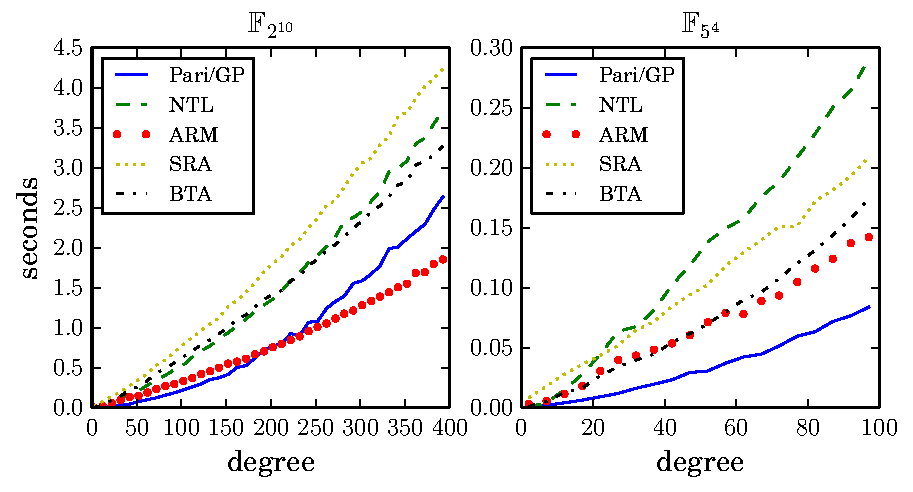
\includegraphics[width=0.55\textwidth]{benchmark}
  \caption{Timings in seconds for $\ff{2^{10}}$ (left) and $\ff{5^4}$
    (right). Abscissa is polynomial degree.}
  \label{fig:benchmarks}
\end{figure}

We used the versions of Pari/GP (v2.7.1) and NTL (v6.1.0) shipped in
the latest Sage distribution (v6.4.1). It should be noted that this is
not the latest NTL version, however we are not aware of any
performance improvements in the latest version (v8.0) concerning root
finding. It is also worth mentioning that the implementation of
polynomials over $\extf$ in Sage 6.4 is backed by the NTL library
(more precisely, by the multi-precision type \texttt{ZZ\_pEX}), thus
the performance of our implementation is essentially to be compared
with NTL's one.

To the best of our knowledge, both Pari/GP and NTL implement the
variant of Cantor-Zassenhaus~\cite{cantor1981} described
in~\cite{GathenS92}. The difference in performances is likely best
explained by the fact that the NTL type \texttt{ZZ\_pEX} is not the
best fit for small characteristic, while Pari/GP optimizes the field
element representation in this case. The fact that our own
implementations performed between the two, and sometimes even better,
shows that these algorithms are practical. However, the observed
differences in performance being so small, they are more likely
attributed to differences in the specific implementation, rather than
to the algorithms themselves.

We conclude that the algorithms reviewed in this paper are of
practical interest for finding polynomial roots in small
characteristic finite fields. In some cases, this in contrast with
what was previously thought, e.g., for ARM. Although general purpose
libraries will probably find no interest in implementing these
algorithms alongside the classical Cantor-Zassenhaus method, they may
turn out to have useful applications in particular finite field
problems.



\section{Conclusion }

In this paper, we revisited several algorithms for root-finding over finite fields of small characteristic. We provided variants of ARM and SRA with an improved average time complexity, and showed that these two algorithms are in a sense dual of each other. We also detailed the relationship between ARM and the well-known BTA. We finally implemented all these algorithms in Sage, showing that all these algorithms perform equally well in practice up to a small constant factor.

\paragraph{Aknowledgements} Luca De Feo would like to thank the
Pari/GP team for kindly hosting him in Bordeaux during the preparation
of the paper, and for giving him useful insights on the internals of
Pari/GP. He also thanks Jean-Pierre Flori for his invaluable help
figuring out the gory details of the Sage/NTL interface.

\scriptsize
\bibliography{refs}
\bibliographystyle{plain}

\end{document}



% Local Variables:
% ispell-local-dictionary:"american"
% End:


%  LocalWords:  affine subspaces linearized factorizations
%  LocalWords:  iteratively
